\documentclass[conference]{IEEEtran}
\IEEEoverridecommandlockouts

\usepackage{cite}
\usepackage{amsmath,amssymb,amsfonts}
\usepackage{amsthm}
\usepackage{algorithm}
\usepackage{algorithmic}
\usepackage{graphicx}
\usepackage{textcomp}
\usepackage{xcolor}
\usepackage{booktabs}
\usepackage{multirow}
\usepackage{array}
\usepackage[hidelinks]{hyperref}

\newtheorem{theorem}{Theorem}
\newtheorem{proposition}{Proposition}
\newtheorem{assumption}{Assumption}

\newcommand{\PH}[1]{{\color{red}\textbf{[#1]}}}

\begin{document}

\title{\LARGE \bf
The Topological Cage: Search-Free Geometric Injection and \\
Multi-Homotopy Routing on a Bounded Medial Manifold
}

\author{Shubham Puri Goswami$^{1}$ and Ravi Prakash$^{2}$%
\thanks{$^{1,2}$Department of Cyber Physical Systems, Indian Institute of Science, Bengaluru, India. {\tt\small \{shubhampg, ravipr\}@iisc.ac.in}}%
}

\maketitle
\thispagestyle{empty}
\pagestyle{empty}

% ==========================================
\begin{abstract}
Medial-axis and generalized Voronoi representations offer a compact, maximum-clearance routing backbone, but two defects hinder standalone use. The \emph{injection problem}: connecting off-skeleton terminals typically requires the very grid search the skeleton was meant to replace. The \emph{Voronoi void}: wide open regions and free-standing obstacles yield sparse or disconnected skeletons because the axis requires equidistance to multiple boundaries.

We propose the \emph{Topological Cage}, closing the medial axis into a bounded, connected manifold. A tangent--gradient parallelism test identifies the ridge's structured interior to fix a clearance scale $C_{\max}$. Truncating the ridge at $d_{\mathrm{cage}}=C_{\max}+\Delta$ and unioning it with that distance level set guarantees connectedness. Terminals attach via bidirectional normalized gradient integration; being eikonal, integral curves cross the cage transversally and terminate within bounded length without grid expansion. The released budget funds homotopy enumeration with lexicographic bottleneck selection. Across four benchmarks, three complex maps, and physical trials, closure reduces graph components from $21$ to $5$, raising feasibility from $24.0\%$ to $99.6\%$ of attainable. Gradient injection attaches $100\%$ of terminals collision-free in $60.7$ steps (vs.\ $2{,}443$ cell expansions for grid search). A damped band cuts integrated curvature by $85.2\%$.
\end{abstract}

% ==========================================
\begin{figure}[!t]
\centerline{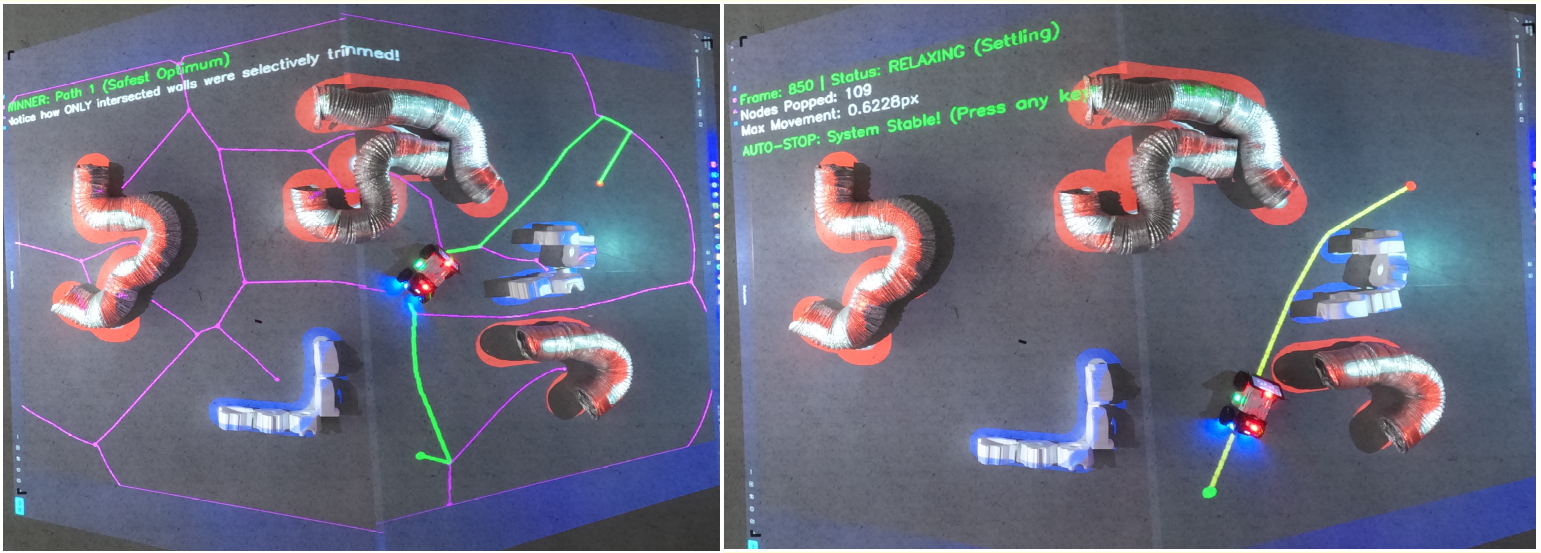
\includegraphics[width=\columnwidth]{hardware_omniwheel.png}}
\caption{Physical execution on an omnidirectional platform. \textbf{Left:} Cage (magenta) with selected homotopy class as raw skeletal route (green). Clearance shells thin only on obstacle components the route contacts. \textbf{Right:} Route after damped-band tensioning (yellow). The band rests against selectively relaxed thresholds, avoiding over-repulsion. Planned planar paths execute without kinematic conversion on the holonomic base.}
\label{fig:hardware}
\end{figure}

% ==========================================
\section{Introduction}

Mobile robots navigating cluttered environments repeatedly solve start-to-goal queries on largely static maps. Grid search is resolution-complete but scales with explored area and hugs boundaries unless manually inflated. Sampling planners handle high dimensions well, but narrow doorways and traps demand sampling densities that erode this advantage.

Distance-field skeletons precompute the maximum-clearance locus, offering clearance by construction and vastly smaller graphs~\cite{lau2013,oleynikova2018,qi2022pruned}. Recent work enables online updates~\cite{lau2013} and contour integration (EGVG)~\cite{qi2025egvg}. However, two problems remain:

\textbf{The injection problem.} Query points rarely lie on the skeleton. Nearest-pixel projection frequently cuts through obstacles ($2.1\%$ of cases here). Inserting queries as temporary obstacles forces skeleton rebuilds. Running A$^\star$ to hit a skeleton pixel reintroduces grid expansion. Raycasting~\cite{qi2025egvg} is fast but line-of-sight dependent.

\textbf{The Voronoi void.} In expansive rooms or around islands, the equidistance locus becomes sparse or disconnected. Across our benchmarks, this fragmentation splits the skeleton into $21$ components, resolving only $24.0\%$ of queries in spaces where $93.0\%$ are attainable.

Both defects stem from using an \emph{unbounded, possibly disconnected} set. Our Topological Cage makes the routing structure \emph{bounded and connected}. A tangent--gradient test sets the internal clearance scale $C_{\max}$; we truncate the ridge at $d_{\mathrm{cage}}=C_{\max}+\Delta$ and union it with the $\{\Psi=d_{\mathrm{cage}}\}$ level set. Truncated ends lie exactly on this level set, fastening components together. Gradient integration from any free point guarantees transversal intersection with the cage, eliminating search during injection. 

\textbf{Contributions.} (i) A bounded medial manifold unifying the routing structure and raising feasibility to $99.6\%$ of attainable. (ii) Search-free bidirectional gradient injection attaching $100\%$ of terminals. (iii) A lexicographic bottleneck criterion refining min-clearance selection. (iv) A damped spring--mass band with per-obstacle relaxation reducing curvature by $85.2\%$. Fig.~\ref{fig:framework} outlines the framework.

% ==========================================
\begin{figure}[!t]
\centerline{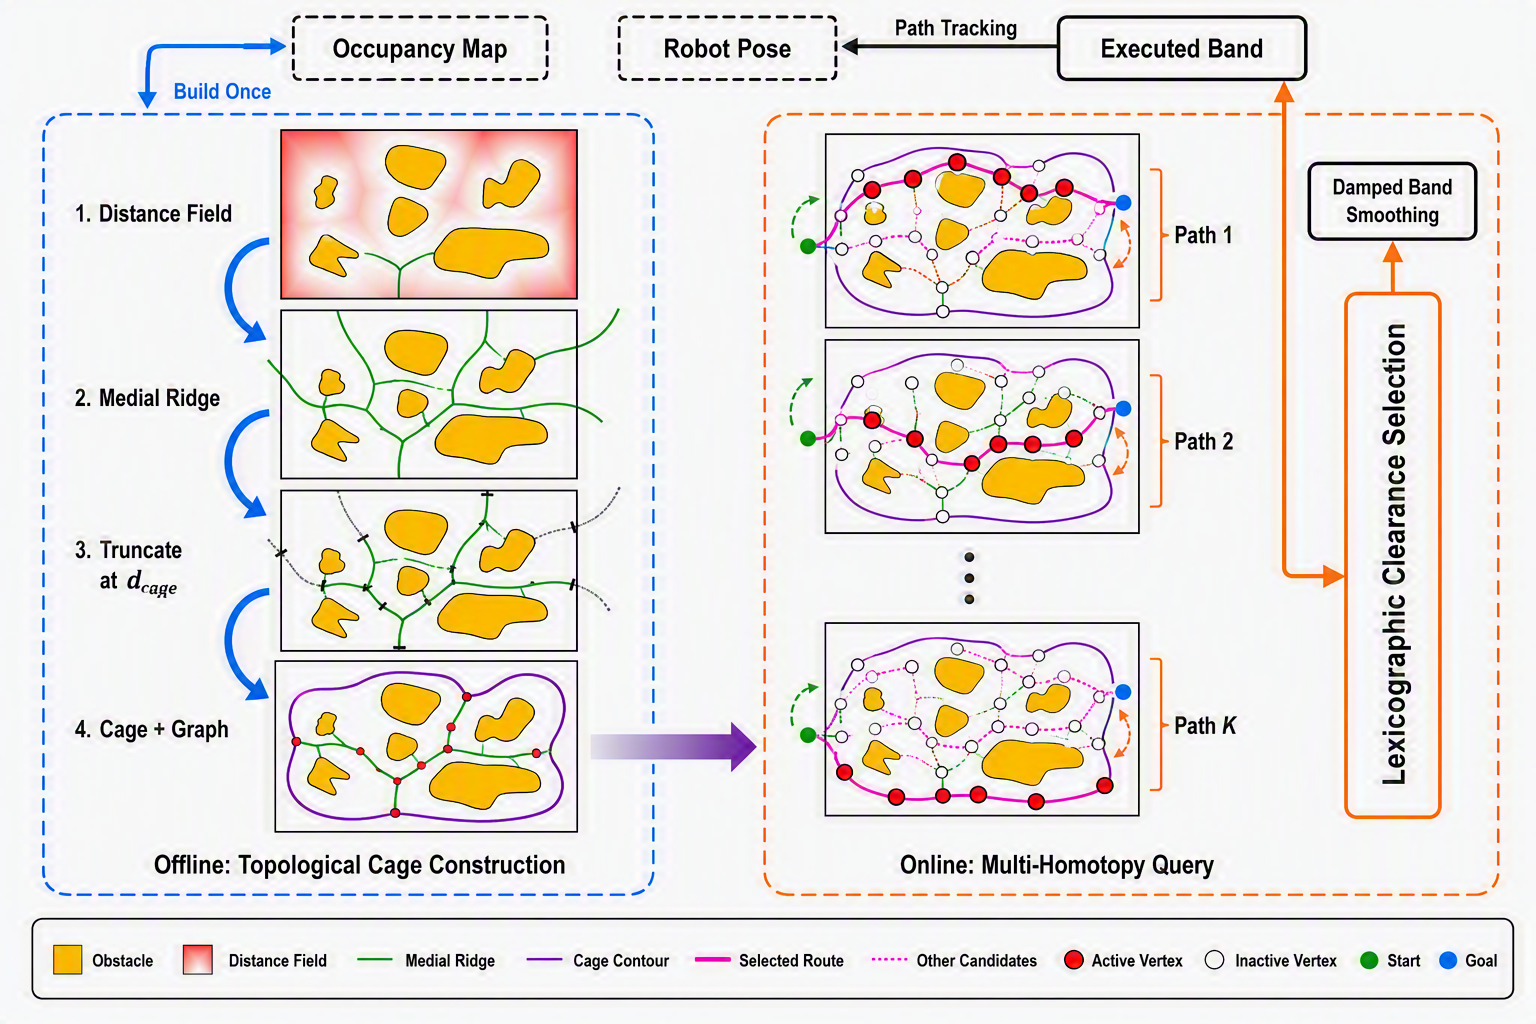
\includegraphics[width=\columnwidth]{Designer.png}}
\caption{Planning framework. \textbf{Left (offline):} The distance field induces the medial ridge. The tangent--gradient test fixes $C_{\max}$. The ridge truncates at $d_{\mathrm{cage}}=C_{\max}+\Delta$ (ticks mark cut points exactly on the level set), forming the Topological Cage. \textbf{Right (online):} Bidirectional scouts attach terminals without grid expansion. $K$ topological candidates (differing in junction sequence) are enumerated. Lexicographic selection isolates the safest route for damped-band smoothing.}
\label{fig:framework}
\end{figure}

% ==========================================
\section{Related Work}

\textbf{Search, sampling and skeletons.} Grid planners~\cite{hart1968,koenig2005} optimize length, not clearance, and scale with area. PRM~\cite{kavraki1996} amortizes costs, but narrow passages require dense sampling. Skeletons (GVD/GVG) extract the distance ridge~\cite{lau2013,hoff1999} for RRT heuristics~\cite{chi2022} or aerial planning~\cite{oleynikova2018}. Skeleton simplification via angle criteria~\cite{foskey2003} discards structure; our tangent--gradient test instead selects a bounding \emph{level}. EGVG~\cite{qi2025egvg} adds contours at user-chosen distances for expressiveness and raycasts for connection. Conversely, we use a single, map-derived contour to guarantee topological closure, enabling search-free gradient connection.

\textbf{Optimization and homotopy.} Elastic bands~\cite{quinlan1993} balance contraction and repulsion but can freeze in tight corridors or suffer node clumping. We address this via selective relaxation and a rest-length penalty. Homotopy enumeration typically uses vertex suppression or distinctness heuristics~\cite{bhattacharya2012,qi2025egvg}. We leverage $K$-shortest paths~\cite{yen1971} and introduce a lexicographic clearance order to deterministically select the safest route.

% ==========================================
\section{Problem Formulation}
\label{sec:problem}

Let $\mathcal{W}\subset\mathbb{R}^2$ be a bounded workspace on a grid of resolution $r$, $\mathcal{O}$ the closed obstacle set, and $\Omega=\mathcal{W}\setminus\mathcal{O}$. The robot radius is $\rho$. Let $\Psi(p)$ be the Euclidean distance to $\partial\mathcal{O}$ and $\hat{n}=\nabla\Psi/\|\nabla\Psi\|$. $\mathcal{M}$ is the medial ridge with unit tangent $\hat{t}_{\mathcal{M}}$. $\mathcal{M}_{\mathrm{int}}$ is the structured interior defined by angular tolerance $\tau$. Let $C_{\max}=\sup_{\mathcal{M}_{\mathrm{int}}}\Psi$ and $d_{\mathrm{cage}}=C_{\max}+\Delta$. The cage is $\mathcal{C}=\mathcal{M}_{\mathrm{trunc}}\cup\mathcal{B}$ where $\mathcal{M}_{\mathrm{trunc}}=\{p\in\mathcal{M}:\Psi(p)\le d_{\mathrm{cage}}\}$ and $\mathcal{B}=\{\Psi=d_{\mathrm{cage}}\}$, with sparse graph $G=(V,E)$. 

\begin{assumption}
\label{asm:setting}
The map is static, $\partial\mathcal{O}$ is known, and $\Omega$ is bounded and connected. $\Psi$ is an exact Euclidean distance transform~\cite{felzenszwalb2012} (1-Lipschitz, $\|\nabla\Psi\|=1$ where differentiable). The offset is admissible: $C_{\max}<d_{\mathrm{cage}}<\sup_{\Omega}\Psi$.
\end{assumption}

We address four problems: \textbf{(P1)} Attach terminals $p_S,p_G\notin\mathcal{M}$ without area-scaled searches. \textbf{(P2)} Unify disjoint skeletons without heuristic bridging. \textbf{(P3)} Deterministically select the safest route among $K$ candidates. \textbf{(P4)} Smooth skeletal routes while avoiding repulsion-freeze and node clumping.

% ==========================================
\section{Offline Construction}
\label{sec:offline}

\subsection{Distance Field and Tangent--Gradient Test}

We compute $\Psi(p)=\min_{q\in\partial\mathcal{O}}\|p-q\|_2$, which solves $\|\nabla\Psi\|=1$ on $\Omega\setminus\mathcal{M}$ and is non-differentiable on $\mathcal{M}$, where gradient direction jumps. The medial ridge is:
\begin{equation}
\mathcal{M}=\{p\in\Omega \mid \exists\, p_i,p_j\in N(p):\ \nabla\Psi(p_i)\cdot\nabla\Psi(p_j)<0\}
\label{eq:ridge}
\end{equation}
$\mathcal{M}$ is connected but unbounded in clearance, extending into open spaces (Fig.~\ref{fig:raw_medial_axis}). Retaining only the structured corridors fragments it.

Inside corridors, the medial curve parallels flanking walls, making the gradient near-orthogonal to the skeleton tangent. On exterior branches, this breaks down. Using $\theta(p)=|90^\circ-\arccos|\hat{t}_{\mathcal{M}}(p)\cdot\hat{n}(p)||$, the structured interior is:
\begin{equation}
\mathcal{M}_{\mathrm{int}}=\big\{p\in\mathcal{M}\ \big|\ |\hat{t}_{\mathcal{M}}(p)\cdot\hat{n}(p)|\le \cos(90^\circ-\tau)\big\}
\label{eq:prune}
\end{equation}
\textbf{This test selects a level, not a membership.} We use $\mathcal{M}_{\mathrm{int}}$ solely to compute $C_{\max}$. Eq.~\eqref{eq:trunc} retains \emph{all} ridge points below the cage level. Because inter-island corridors stay locally parallel, a single scalar $\tau$ registers both wall and island structures (Fig.~\ref{fig:angle_cutoff}). 

\begin{figure}[htbp]
\centerline{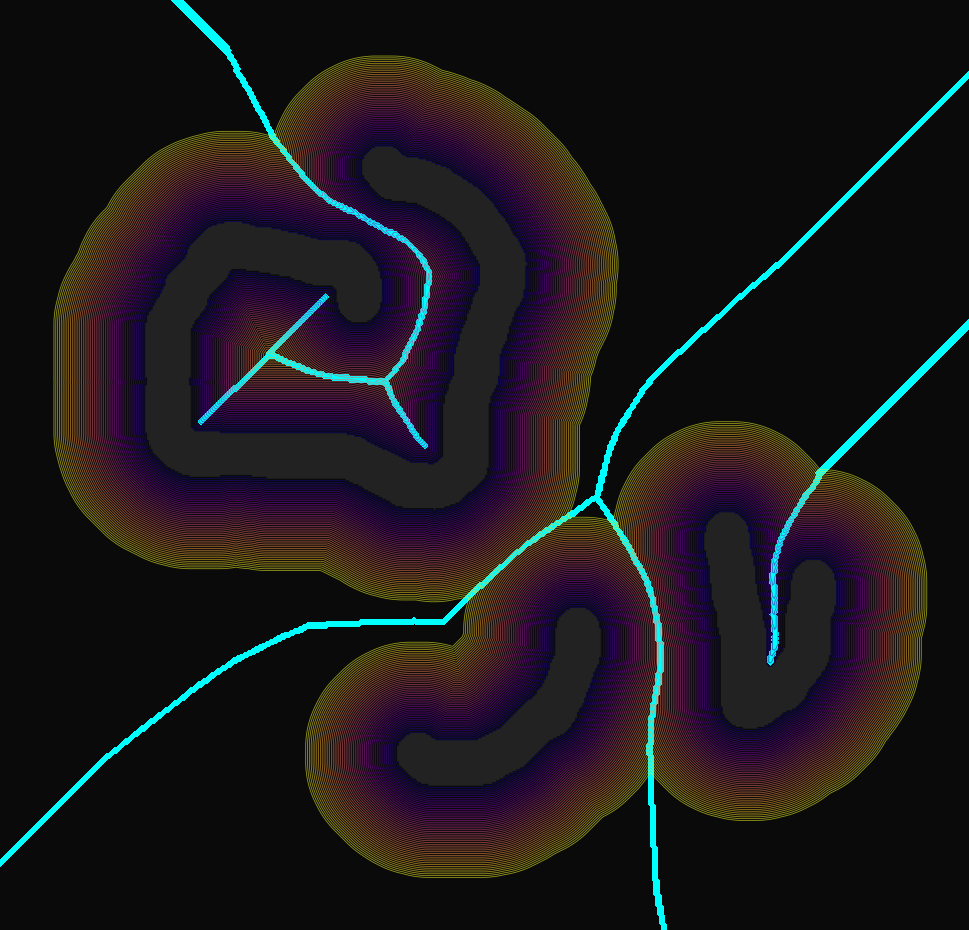
\includegraphics[width=0.85\columnwidth]{infinitemedial.png}}
\caption{The raw medial ridge (cyan) correctly captures corridors but extends infinitely into open space. Retaining only structure fragments the graph.}
\label{fig:raw_medial_axis}
\end{figure}

\begin{figure}[htbp]
\centerline{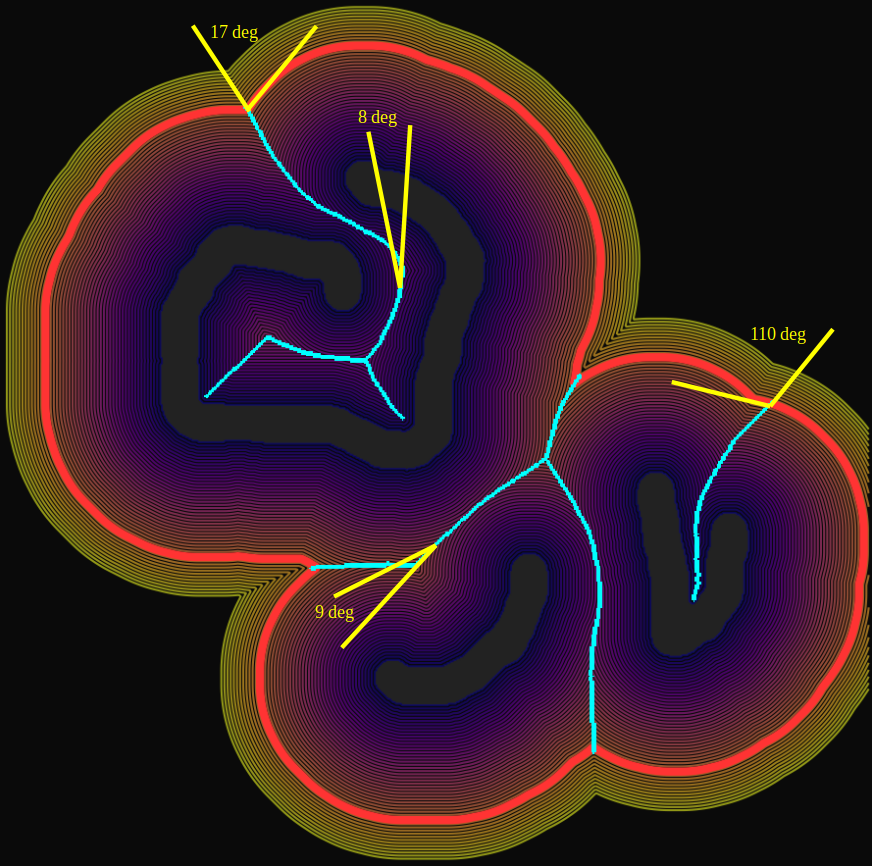
\includegraphics[width=0.85\columnwidth]{angleprunning.png}}
\caption{Tangent--gradient test. Corridors exhibit near-orthogonal pairs ($\theta\!\approx\!8^\circ$). Open-space branches diverge ($\theta\!\approx\!110^\circ$) and are excluded from $\mathcal{M}_{\mathrm{int}}$. Inter-island gaps stay parallel and are accurately captured.}
\label{fig:angle_cutoff}
\end{figure}

\subsection{Closure and Graph Abstraction}
\label{sec:closure}

Setting $C_{\max}=\sup_{p\in\mathcal{M}_{\mathrm{int}}}\Psi(p)$ and $d_{\mathrm{cage}}=C_{\max}+\Delta$:
\begin{align}
\mathcal{M}_{\mathrm{trunc}} &= \{p\in\mathcal{M}: \Psi(p)\le d_{\mathrm{cage}}\} \label{eq:trunc}\\
\mathcal{B} &= \{p\in\Omega: |\Psi(p)-d_{\mathrm{cage}}|\le\varepsilon\}
\end{align}
where $\varepsilon$ is half the grid diagonal. The cage is:
\begin{equation}
\boxed{\ \mathcal{C}=\mathcal{M}_{\mathrm{trunc}}\ \cup\ \mathcal{B}\ }
\label{eq:cage}
\end{equation}
Outward branches truncate precisely at $\Psi=d_{\mathrm{cage}}$, leaving cut ends exactly on $\mathcal{B}$, binding the structure (Theorem~\ref{thm:connected}). $\mathcal{C}$ compresses into graph $G=(V,E)$ via pixel-degree classification~\cite{lau2013}. Pixels below $\rho+\delta_{\mathrm{safe}}$ are discarded offline, eliminating query-time collision checks. Graph sizes reflect topology, yielding roughly $1000\times$ compression.

% ==========================================
\section{Online Query: Search-Free Injection}
\label{sec:online}

\subsection{Bidirectional Gradient Scouts}

From $p_S$ (identically $p_G$), we integrate $p_{k+1}=p_k \pm \alpha\,\hat{n}(p_k)$ until contacting $\mathcal{C}$. The $+$ branch (``climber'') ascends clearance; the $-$ branch (``diver'') descends. Both are structurally necessary (Fig.~\ref{fig:scouts}): terminals below the envelope must climb to reach the ridge or $\mathcal{B}$, while terminals enclosed by $\mathcal{B}$ in open voids must dive to recover the envelope. Contacts are inserted as temporary vertices in $G$.

\begin{figure}[htbp]
\centerline{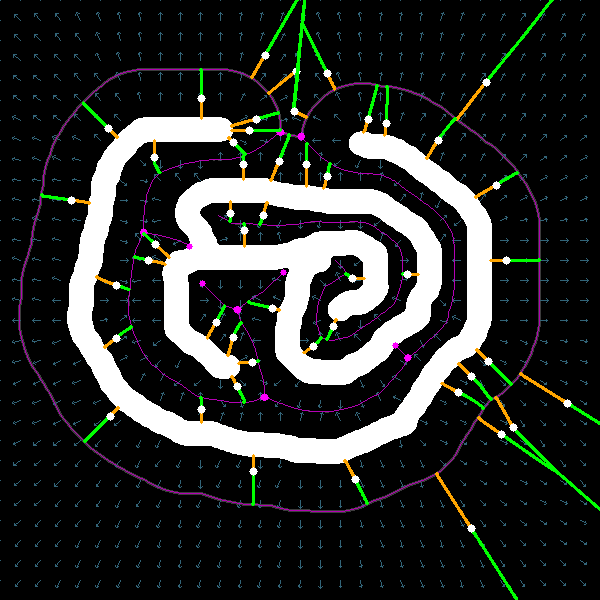
\includegraphics[width=0.85\columnwidth]{scout_navigation_map.png}}
\caption{Injection. The climber (green, $+\hat{n}$) and diver (orange, $-\hat{n}$) integrate until contacting the cage (purple), depending on starting clearance.}
\label{fig:scouts}
\end{figure}

\subsection{Guarantees}

\begin{theorem}[Connectedness]
\label{thm:connected}
Under Assumption~\ref{asm:setting}, $\mathcal{C}=\mathcal{M}_{\mathrm{trunc}}\cup\mathcal{B}$ is connected.
\end{theorem}
\begin{proof}
$\mathcal{M}$ is a connected deformation retract of $\Omega$. Let $\mathcal{B}_j$ be a component of $\{\Psi=d_{\mathrm{cage}}\}$ bounding region $R_j$ where $\Psi>d_{\mathrm{cage}}$. $\Psi$ attains an interior maximum in $R_j$ on $\mathcal{M}$. Since $\mathcal{M}$ connects to the sublevel region, it crosses $\partial R_j=\mathcal{B}_j$ exactly at $d_{\mathrm{cage}}$, placing that point in both $\mathcal{M}_{\mathrm{trunc}}$ and $\mathcal{B}_j$. Any two points in $\mathcal{C}$ joined by $\gamma\subset\mathcal{M}$ stay in $\mathcal{M}_{\mathrm{trunc}}$ when $\Psi\le d_{\mathrm{cage}}$. Excursions into $\{\Psi>d_{\mathrm{cage}}\}$ enter and exit on the same connected $\mathcal{B}_j$, allowing paths entirely within $\mathcal{C}$.
\end{proof}

\begin{theorem}[Finite-length injection]
\label{thm:injection}
For $p_0\in\Omega$ with $\Psi(p_0)>\rho+\delta_{\mathrm{safe}}$, at least one integral curve of $\pm\hat{n}$ contacts $\mathcal{C}$ within arc length $|d_{\mathrm{cage}}-\Psi(p_0)|$.
\end{theorem}
\begin{proof}
Since $\Psi$ is eikonal, $\tfrac{d}{ds}\Psi=\pm 1$ along $\dot{p}=\pm\hat{n}$. Gradient magnitude persists near $\mathcal{M}$ (only direction jumps), ensuring curves cross $\mathcal{M}$ transversally at unit speed. Cycles are monotonically precluded. If $\Psi(p_0)<d_{\mathrm{cage}}$, the climber meets a valid ridge point or reaches $\mathcal{B}$. If $\Psi(p_0)>d_{\mathrm{cage}}$, the diver meets $\mathcal{B}$ before hitting obstacles. Level changes occur at unit rate, bounding length.
\end{proof}

\begin{proposition}[Query cost]
Injection requires at most $\lceil |d_{\mathrm{cage}}-\Psi(p_0)|/\alpha \rceil$ steps, independent of $|\Omega|$. Total cost is $O(\Psi_{\text{span}}/\alpha) + O(K(|E|+|V|\log|V|))$~\cite{yen1971}.
\end{proposition}

% ==========================================
\section{Selection and Smoothing}
\label{sec:opt}

\subsection{Enumeration and Lexicographic Selection}

Using Yen's algorithm~\cite{yen1971}, we enumerate $K$ loopless shortest paths, discarding geometrically redundant variants. Let $P$ have pixel sequence $\{p_1,\dots,p_M\}$ and sorted clearance profile $\sigma(P)=(\Psi_{(1)},\dots,\Psi_{(M)})$. We define $P\succ P'$ iff $\sigma(P)$ is lexicographically greater, and select $P^\star=\arg\max_{\succ}\{P_1,\dots,P_K\}$. The first component is minimum clearance, maximizing the tightest bottleneck. Refinement acts on ties, comparing subsequent bottlenecks deterministically (Fig.~\ref{fig:lexicographical}).

\begin{figure}[htbp]
\centerline{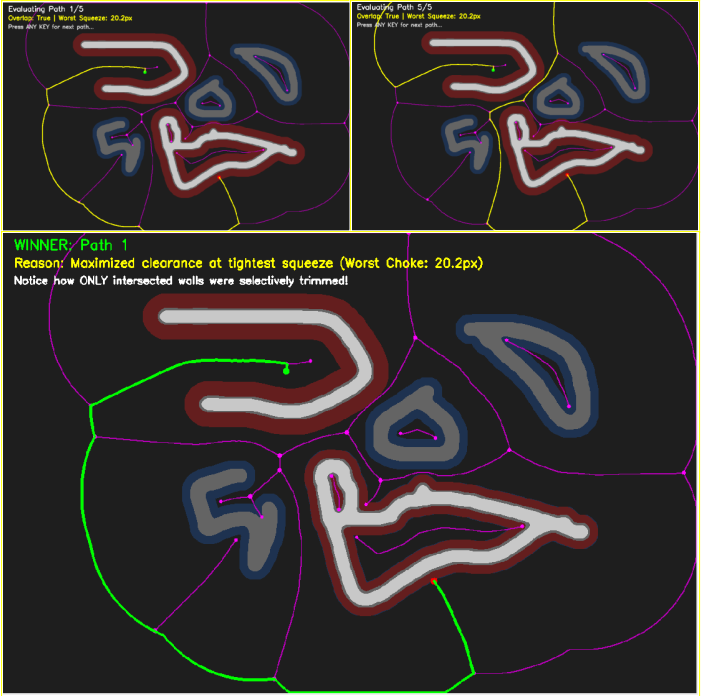
\includegraphics[width=\columnwidth]{pathcomp.png}}
\caption{Lexicographic selection. $K$ topological candidates are enumerated; annotations show sorted clearance heads. The selected route (bottom right) maximizes the tightest and second-tightest passages, prioritizing safety over length.}
\label{fig:lexicographical}
\end{figure}

\subsection{Selective Relaxation and Damped Band}

A uniform repulsion threshold paralyzes bands in tight passages. We label obstacle components $\{O_m\}$ with fields $\Psi_O$ and track $s_O=\min_{p\in P^\star}\Psi_O(p)$. We relax thresholds only for intersecting components:
\begin{equation}
\tau_O=\min\big(\tau_O^{\mathrm{nom}},\ \max(s_O-\eta,\ \rho+\delta_{\mathrm{safe}})\big)
\label{eq:relax}
\end{equation}
Safety is preserved by clamping to $\rho+\delta_{\mathrm{safe}}$. Discretizing $P^\star$ into nodes $\{P_i\}$, dynamics are governed by:
\begin{align}
\ddot{P}_i &= W_s \vec{F}^{\,s}_i + W_r \vec{F}^{\,r}_i - D\,\dot{P}_i \label{eq:dyn} \\
\vec{F}^{\,s}_i &= \sum_{j\in\{i\pm1\}}\frac{P_j-P_i}{\|P_j-P_i\|}\big(\|P_j-P_i\|-d_{\mathrm{rest}}\big) \nonumber \\
\vec{F}^{\,r}_i &= \sum_{O} \frac{\nabla\Psi_O(P_i)}{\|\nabla\Psi_O(P_i)\|}\big[\tau_O-\Psi_O(P_i)\big]_+ \nonumber
\end{align}
The rest length $d_{\mathrm{rest}}$ prevents node clumping, while damping $D$ eliminates oscillation. We apply distributed decimation (removing every $N_{\mathrm{pop}}$-th node globally) to avoid local freezing. Nodes are clamped to $\Psi(P_i)\ge\rho+\delta_{\mathrm{safe}}$ post-update.

\begin{algorithm}[htbp]
\caption{Topological Cage query}
\label{alg:query}
\begin{algorithmic}[1]
\STATE \textbf{Offline:} $\Psi\!\leftarrow\!\mathrm{EDT}(\Omega)$; $\mathcal{M}\!\leftarrow\!\mathrm{ridge}(\Psi)$
\STATE $\mathcal{M}_{\mathrm{int}}\!\leftarrow\!$ Eq.~\eqref{eq:prune}; $C_{\max}\!\leftarrow\!\sup\Psi|_{\mathcal{M}_{\mathrm{int}}}$; $d_{\mathrm{cage}}\!\leftarrow\!C_{\max}\!+\!\Delta$
\STATE $\mathcal{C}\!\leftarrow\!\mathcal{M}_{\mathrm{trunc}}\cup\{\Psi\!=\!d_{\mathrm{cage}}\}$; $G\!\leftarrow\!\mathrm{abstract}(\mathcal{C})$
\STATE \textbf{Online:} integrate $p_{k+1}=p_k\pm\alpha\hat{n}$ from $p_S,p_G$; insert
\STATE $\{P_1..P_K\}\leftarrow\mathrm{Yen}(G,p_S',p_G',K)$; $P^\star\leftarrow$ lex-max $\sigma(P_k)$
\STATE $\{\tau_O\}\leftarrow$ Eq.~\eqref{eq:relax} on $P^\star$
\STATE \textbf{if} all candidates need $\tau_O$ at floor \textbf{then return} unresolved
\STATE iterate Eq.~\eqref{eq:dyn} with decimation until $v_{\max}<\epsilon_{\mathrm{stab}}$
\end{algorithmic}
\end{algorithm}

% ==========================================
\section{Experimental Setup}
\label{sec:setup}

\textbf{Implementation.} Python (single-thread Ryzen 5 5500U). Parameters: $\tau=17^\circ$, $\Delta=20$~px, $\alpha=0.5$~px, $K=5$, max overlap $0.85$, $r=0.02$~m/px, $\rho+\delta_{\mathrm{safe}}=6$~px ($0.12$~m), $\tau^{\mathrm{nom}}_{\mathrm{rigid}}=30$~px, $\tau^{\mathrm{nom}}_{\mathrm{soft}}=15$~px, $\eta=2$~px, $d_{\mathrm{rest}}=5$~px, initial spacing $8$~px, $W_s=0.55$, $W_r=2.5$, $D=0.4$, $h=1.0$, $\epsilon_{\mathrm{stab}}=0.7$~px/iter.

\textbf{Environments.} Four $500\times750$~px benchmarks ($150$~m$^2$): \textbf{E1} (indoor), \textbf{E2} (open void), \textbf{E3} (islands), \textbf{E4} (trap). Three complex maps (spirals, concave islands, maze) provide case studies.

\textbf{Baselines.} Grid A$^\star$~\cite{hart1968} (also used as attainability oracle); PRM~\cite{kavraki1996} ($2500$ samples); RRT$^\star$~\cite{karaman2011}; GVD with A$^\star$ injection; FMM; and a DWA-style planner~\cite{fox1997}. EGVG raycast is evaluated as ablation A2c.

\textbf{Protocol.} $Q=100$ random pairs per environment ($400$ total), sampled in free space ($\ge 120$~px distance). Evaluated on offline/online cost, feasibility, and clearance.

% ==========================================
\section{Results}
\label{sec:results}

\subsection{Overall Comparison}

Table~\ref{tab:master} shows feasibility sharply dividing methods. GVD resolves only $33.5\%$ due to skeleton disconnections, while our caged routing resolves $92.8\%$. Our routing takes $24.7$~ms versus A$^\star$'s $250.2$~ms ($10\times$ faster). Over 100 queries, our total time (including offline cost) breaks even against A$^\star$ at 2 queries. PRM is faster ($8.2$~ms) but requires $945.5$~ms offline and ignores corridor clearance. In the maze benchmark, our planner visits $98$ nodes versus $244{,}021$ for A$^\star$, maintaining $14$~px clearance safely away from boundaries.

\begin{table*}[htbp]
\caption{Consolidated comparison. Left: E1--E4 ($Q=400$). Right: maze case study. Best per column in bold.}
\label{tab:master}
\begin{center}
\begin{tabular}{@{}l cccc c cccc@{}}
\toprule
& \multicolumn{4}{c}{\textbf{Benchmark suite E1--E4 ($Q=400$)}} & & \multicolumn{4}{c}{\textbf{Maze case study (single query)}} \\
\cmidrule(lr){2-5} \cmidrule(lr){7-10}
\textbf{Method} & \textbf{Offline} & \textbf{Query} & \textbf{Total 100q} & \textbf{Resolved} & & \textbf{Nodes/cells} & \textbf{Clearance} & \textbf{Time} & \textbf{Success} \\
 & (ms) & (ms) & (s) & (\%) & & \textbf{visited} & (px) & (ms) & \\ \midrule
A$^\star$~\cite{hart1968}              & $\mathbf{0.0}$ & $250.2$ & $25.02$ & $\mathbf{93.0}$ & & $244{,}021$ & $1.0$ & $3695.99$ & yes \\
RRT$^\star$~\cite{karaman2011}         & $\mathbf{0.0}$ & $117.6$ & $11.76$ & $92.5$ & & $1{,}191$ & $0.0$ & $473.77$ & no \\
PRM (dense)~\cite{kavraki1996}         & $945.5$ & $\mathbf{8.2}$ & $1.77$ & $84.3$ & & $1{,}002$ & $3.0$ & $430.76$ & yes \\
FMM                                    & --- & --- & --- & --- & & $360{,}000$ & $0.0$ & $176.22$ & no \\
GVD + A$^\star$ inject                 & $114.7$ & $17.4$ & $1.85$ & $33.5$ & & --- & --- & --- & --- \\ \midrule
\textbf{Ours} (global routing)         & $343.9$ & $24.7$ & $\mathbf{2.81}$ & $92.8$ & & $\mathbf{98}$ & $\mathbf{14.0}$ & $\mathbf{28.38}$ & \textbf{yes} \\
\textbf{Ours} (routing $+$ band)       & $343.9$ & $84.7$ & $8.81$ & $92.8$ & & --- & --- & --- & --- \\ \bottomrule
\end{tabular}
\end{center}
\footnotesize Normalized against A$^\star$ attainability, our feasibility is $99.6\%$ (Table~\ref{tab:perenv}). Dashes indicate omissions due to prohibitive execution (FMM batch), topological failure (GVD maze), or inapplicability.
\end{table*}

\subsection{Per-Environment Evidence}

Table~\ref{tab:perenv} shows caging reduces raw components from $21$ to $5$. E2--E4 condense to single components, fulfilling Theorem~\ref{thm:connected}, driving feasibility from $24.0\%$ to $92.8\%$. In open voids (E2) and islands (E3), uncaged feasibility hits $7\%$ and $13\%$, while the cage achieves $100\%$. Across $400$ queries, our method missed only one attainable path ($99.6\%$ normalized success). 

\begin{table}[htbp]
\caption{Per-environment closure, feasibility, graph size, and query cost}
\label{tab:perenv}
\begin{center}
\setlength{\tabcolsep}{3.5pt}
\begin{tabular}{@{}lcccccccc@{}}
\toprule
& \multicolumn{2}{c}{\textbf{Components}} & \multicolumn{3}{c}{\textbf{Feasibility (\%)}} & \multicolumn{3}{c}{\textbf{Query cost (ms)}} \\
\cmidrule(lr){2-3} \cmidrule(lr){4-6} \cmidrule(lr){7-9}
\textbf{Env} & raw & caged & attain. & raw & caged & inject & enum & tension \\ \midrule
E1 & $8$ & $2$ & $72$ & $25.0$ & $71.0$ & $1.49$ & $30.83$ & $63.78$ \\
E2 & $4$ & $\mathbf{1}$ & $100$ & $7.0$ & $\mathbf{100.0}$ & $4.43$ & $15.97$ & $45.86$ \\
E3 & $6$ & $\mathbf{1}$ & $100$ & $13.0$ & $\mathbf{100.0}$ & $1.60$ & $28.01$ & $42.71$ \\
E4 & $3$ & $\mathbf{1}$ & $100$ & $51.0$ & $\mathbf{100.0}$ & $1.12$ & $13.71$ & $61.93$ \\ \midrule
Mean & $21$ & $\mathbf{5}$ & $93$ & $24.0$ & $\mathbf{92.8}$ & $2.16$ & $22.13$ & $53.57$ \\ \bottomrule
\end{tabular}
\end{center}
\footnotesize Graph sizes $|V|/|E|$: E1 $116/163$, E2 $52/75$, E3 $75/114$, E4 $44/61$.
\end{table}

\subsection{Component Contributions}

Table~\ref{tab:ablation} isolates module impact. Uncaged routing feasibility plummets to $26.3\%$. Gradient injection uniquely achieves $100\%$ attachment with zero collisions. A$^\star$ scales poorly ($2{,}443$ cell expansions vs.\ $60.7$ gradient steps). Bidirectional scouts partition the space effectively: in E2, climbers attach $73.8\%$ and divers $27.5\%$. Lexicographic selection outperforms shortest-length by $3.0\%$ and cuts ties ($247\rightarrow107$). The full elastic band cuts integrated curvature by $85.2\%$ and spacing dispersion by $97.4\%$. Damping proves critical: omitting it spikes curvature $39\times$.

\begin{table}[htbp]
\caption{Component contributions (mean over E1--E4)}
\label{tab:ablation}
\begin{center}
\setlength{\tabcolsep}{4pt}
\begin{tabular}{@{}llccc@{}}
\toprule
\textbf{ID} & \textbf{Variant} & \textbf{Feas.\ \%} & \textbf{Min clr (m)} & \textbf{Cost} \\ \midrule
A1 & no closure & $26.3$ & $0.910$ & $45.4$~ms \\ \midrule
\multicolumn{5}{@{}l}{\textit{A2 --- injection mechanism (attachment \%, collisions)}} \\
A2a & nearest-pixel & $100.0$ & \multicolumn{2}{c}{$2.1\%$ collide, $0.879$~ms} \\
A2b & A$^\star$ to skeleton & $100.0$ & \multicolumn{2}{c}{$2443$ cells, $3.182$~ms} \\
A2c & raycast~\cite{qi2025egvg} & $98.4$ & \multicolumn{2}{c}{$0\%$ collide, $\mathbf{0.079}$~ms} \\
-- & \textbf{gradient (ours)} & $\mathbf{100.0}$ & \multicolumn{2}{c}{$\mathbf{0\%}$ collide, $60.7$ steps} \\ \midrule
\multicolumn{5}{@{}l}{\textit{A3 --- scout branches (attachment over 320 terminals)}} \\
A3 & climber only & $93.4$ & $0.870$ & $83.8$\% routed \\
A3 & diver only & $9.1$ & --- & $0.0$\% routed \\
-- & \textbf{both} & $\mathbf{100.0}$ & $0.854$ & $\mathbf{94.4}$\% routed \\ \midrule
\multicolumn{5}{@{}l}{\textit{A4 --- selection criterion (375 multi-candidate queries)}} \\
A4 & shortest length & $0.972$ & $1.530$ mean & $1$ tie \\
A4 & max min-clr & $\mathbf{1.001}$ & $1.557$ mean & $247$ ties \\
-- & \textbf{lexicographic} & $\mathbf{1.001}$ & $\mathbf{1.588}$ mean & $\mathbf{107}$ ties \\ \midrule
\multicolumn{5}{@{}l}{\textit{A5 --- band terms ($\int|\kappa|ds$, spacing CV, settled \%)}} \\
A5 & raw skeletal & $26.96$ & $3.810$ & --- \\
A5 & no damping & $155.11$ & $0.648$ & $2.5$ \\
A5 & no relaxation & $5.48$ & $0.185$ & $67.5$ \\
A5 & end decimation & $3.94$ & $0.174$ & $\mathbf{86.9}$ \\
A5 & no rest length & $\mathbf{2.77}$ & $0.153$ & $70.6$ \\
-- & \textbf{full} & $3.98$ & $\mathbf{0.101}$ & $83.8$ \\ \bottomrule
\end{tabular}
\end{center}
\end{table}

\subsection{Parameter Sensitivity and Complex Environments}

Table~\ref{tab:sweep} confirms feasibility remains $91.3\%$ across wide bounds of $\tau\in[8^\circ,45^\circ]$ and $\Delta\in[5,80]$~px. Clearance saturates at $K=3$. Fig.~\ref{fig:casestudy} demonstrates $K=5$ enumeration and successful lexicographic selection on three complex case studies.

\begin{table}[htbp]
\caption{Parameter sensitivity, mean over E1--E4}
\label{tab:sweep}
\begin{center}
\setlength{\tabcolsep}{2pt}
\begin{tabular}{@{}lccccc@{}}
\toprule
\textbf{$\tau$ (deg)} & $8$ & $12$ & $17$ & $30$ & $45$ \\
Feas.\ \% / min clr & $91.3/.901$ & $91.3/.863$ & $91.3/.854$ & $91.3/.841$ & $91.3/.839$ \\ \midrule
\textbf{$\Delta$ (px)} & $5$ & $10$ & $20$ & $40$ & $80$ \\
Feas.\ \% / min clr & $91.3/.886$ & $91.3/.852$ & $91.3/.854$ & $91.3/.850$ & $91.3/.884$ \\ \midrule
\textbf{$K$} & $1$ & $3$ & $5$ & $8$ & $12$ \\
Query ms / min clr & $41.0/.839$ & $61.1/.854$ & $62.2/.854$ & $62.2/.854$ & $61.9/.854$ \\ \midrule
\textbf{$\alpha$ (px)} & $0.25$ & $0.5$ & $1.0$ & $2.0$ & $4.0$ \\
Attach \% / steps & $100/123.6$ & $100/62.5$ & $100/32.0$ & $100/16.7$ & $\mathbf{100/9.1}$ \\ \bottomrule
\end{tabular}
\end{center}
\end{table}

\begin{figure*}[htbp]
\centerline{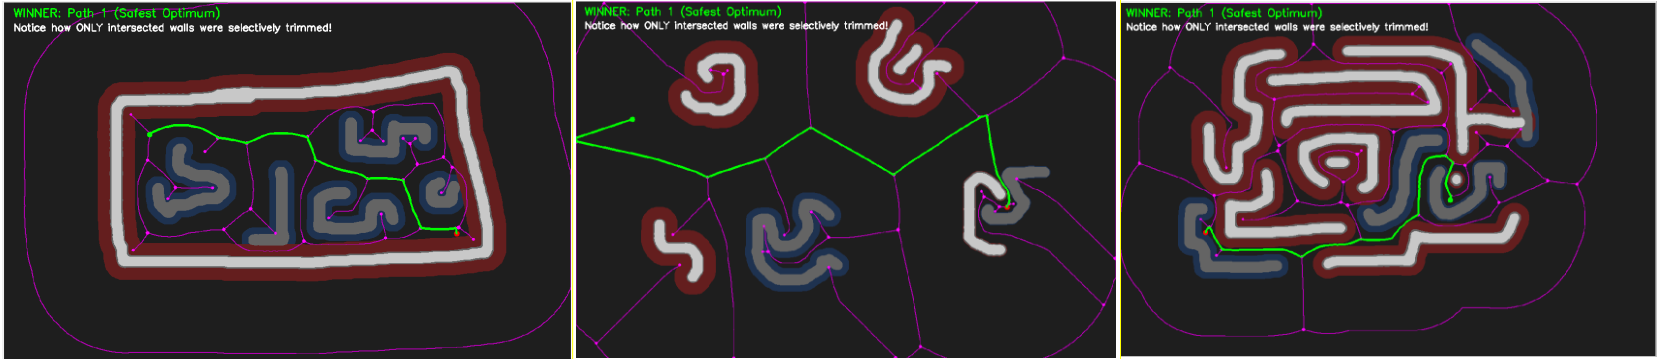
\includegraphics[width=0.96\textwidth]{E134.png}}
\caption{Operator-drawn complex environments. \textbf{Left:} Nested spirals. \textbf{Centre:} Concave islands. \textbf{Right:} Dense maze. In all, the cage (magenta) unifies the skeleton, terminals inject without grid expansion, and lexicographic criteria select the safest route (green) from $K=5$ candidates.}
\label{fig:casestudy}
\end{figure*}

% ==========================================
\section{Limitations and Future Work}
\label{sec:limitations}

\textbf{Global scalar cage level.} $d_{\mathrm{cage}}$ relies on a global supremum ($C_{\max}$). A single wide hallway globally pushes the envelope outward, limiting applications to static maps. Spatially varying cage levels would address this.
\textbf{Discretization sensitivity.} Exact lexicographic comparison is vulnerable to grid aliasing; quantile comparisons could improve robustness.
\textbf{Safety floor.} Clamping nodes discretey ensures safety; interpolated trajectories require swept-segment tests. Kinodynamic limits are deferred.
\textbf{Future work.} Yen's algorithm generates redundant paths requiring post-filtering. Enumerating directly on the cage graph's vertex sequence would yield a topologically complete, non-redundant candidate set.

% ==========================================
\section{Conclusion}

The Topological Cage closes the medial axis using a clearance level fixed by a tangent--gradient test. This unifies fragmented routing structures, raising query feasibility from $24.0\%$ to $99.6\%$ of attainable. Bidirectional gradient integration enables search-free transversal injection, resolving $100\%$ of queries collision-free in $60.7$ steps. This efficiency funds homotopy enumeration, lexicographic safety selection, and a damped elastic band that cuts curvature by $85.2\%$. 

% ==========================================
\appendices
\section{The Voronoi Void}
\label{appendix:voronoi_void}

In open voids or around free-standing islands, skeletons lose corridor-level connections (Fig.~\ref{fig:voronoi_problem}, left). Resolving this via grid search scales poorly ($3{,}068$ expansions in E2). Caging places $\mathcal{B}$ through voids by construction; gradient integration reaches it predictably, uniting the structure without grid searches (Fig.~\ref{fig:voronoi_problem}, right).

\begin{figure}[htbp]
\centerline{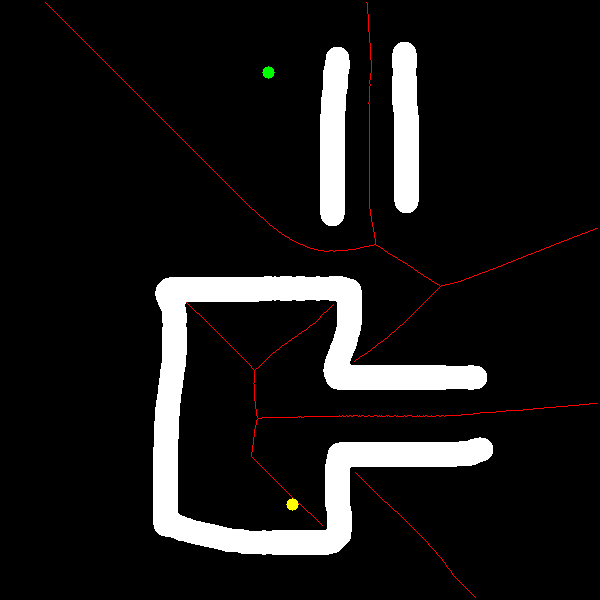
\includegraphics[width=0.48\columnwidth]{voronoi_shortcoming_raw.png}\hfill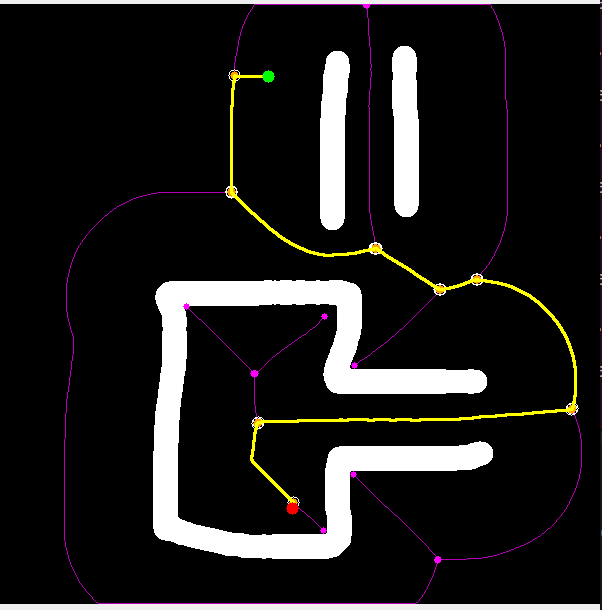
\includegraphics[width=0.48\columnwidth]{voronoi_our_path.png}}
\caption{\textbf{Left:} The standard medial axis (red) leaves the query point (green) disconnected in the Voronoi void. \textbf{Right:} The cage (purple) predictably crosses the void, enabling search-free connection (yellow).}
\label{fig:voronoi_problem}
\end{figure}

% ==========================================
\begin{thebibliography}{00}
\bibitem{qi2025egvg} H. Qi \emph{et al.}, ``Enveloped Generalized Voronoi Graph and multi-topology path planning for navigation in unknown environments,'' \textit{TechRxiv preprint}, Oct.\ 2025.
\bibitem{hart1968} P. E. Hart \emph{et al.}, ``A formal basis for the heuristic determination of minimum cost paths,'' \textit{IEEE Trans. Syst. Sci. Cybern.}, vol. 4, no. 2, pp. 100--107, 1968.
\bibitem{koenig2005} S. Koenig and M. Likhachev, ``Fast replanning for navigation in unknown terrain,'' \textit{IEEE Trans. Robot.}, vol. 21, no. 3, pp. 354--363, 2005.
\bibitem{kavraki1996} L. E. Kavraki \emph{et al.}, ``Probabilistic roadmaps for path planning in high-dimensional configuration spaces,'' \textit{IEEE Trans. Robot. Autom.}, vol. 12, no. 4, pp. 566--580, 1996.
\bibitem{lavalle1998} S. M. LaValle, ``Rapidly-exploring random trees: A new tool for path planning,'' Tech. Rep. TR 98-11, Iowa State Univ., 1998.
\bibitem{karaman2011} S. Karaman and E. Frazzoli, ``Sampling-based algorithms for optimal motion planning,'' \textit{Int. J. Robot. Res.}, vol. 30, no. 7, pp. 846--894, 2011.
\bibitem{felzenszwalb2012} P. F. Felzenszwalb and D. P. Huttenlocher, ``Distance transforms of sampled functions,'' \textit{Theory of Computing}, vol. 8, no. 1, pp. 415--428, 2012.
\bibitem{lau2013} B. Lau \emph{et al.}, ``Efficient grid-based spatial representations for robot navigation in dynamic environments,'' \textit{Robot. Auton. Syst.}, vol. 61, no. 10, pp. 1116--1130, 2013.
\bibitem{hoff1999} K. E. Hoff III \emph{et al.}, ``Fast computation of generalized Voronoi diagrams using graphics hardware,'' in \textit{Proc. SIGGRAPH}, 1999, pp. 277--286.
\bibitem{oleynikova2018} H. Oleynikova \emph{et al.}, ``Sparse 3D topological graphs for micro-aerial vehicle planning,'' in \textit{IEEE/RSJ IROS}, 2018, pp. 1--9.
\bibitem{qi2022pruned} Y. Qi \emph{et al.}, ``Compact and efficient topological mapping for large-scale environment with pruned Voronoi diagram,'' \textit{Drones}, vol. 6, no. 7, p. 183, 2022.
\bibitem{foskey2003} M. Foskey \emph{et al.}, ``Efficient computation of a simplified medial axis,'' in \textit{Proc. ACM Symp. Solid Modeling}, 2003, pp. 96--107.
\bibitem{chi2022} W. Chi \emph{et al.}, ``A generalized Voronoi diagram-based efficient heuristic path planning method for RRTs in mobile robots,'' \textit{IEEE Trans. Ind. Electron.}, vol. 69, no. 5, pp. 4926--4937, 2022.
\bibitem{zhang2024agv} R. Zhang \emph{et al.}, ``Design and practical implementation of a high efficiency two-layer trajectory planning method for AGV,'' \textit{IEEE Trans. Ind. Electron.}, vol. 71, no. 2, pp. 1811--1822, 2024.
\bibitem{yang2022far} F. Yang \emph{et al.}, ``FAR planner: Fast, attemptable route planner using dynamic visibility update,'' in \textit{IEEE/RSJ IROS}, 2022, pp. 9--16.
\bibitem{dobson2014} A. Dobson and K. E. Bekris, ``Sparse roadmap spanners for asymptotically near-optimal motion planning,'' \textit{Int. J. Robot. Res.}, vol. 33, no. 1, pp. 18--47, 2014.
\bibitem{quinlan1993} S. Quinlan and O. Khatib, ``Elastic bands: Connecting path planning and control,'' in \textit{IEEE ICRA}, 1993, pp. 802--807.
\bibitem{rosmann2012} C. R\"osmann \emph{et al.}, ``Trajectory modification considering dynamic constraints of autonomous robots,'' in \textit{7th German Conf.\ Robotics}, 2012, pp. 1--6.
\bibitem{fox1997} D. Fox \emph{et al.}, ``The dynamic window approach to collision avoidance,'' \textit{IEEE Robot. Autom. Mag.}, vol. 4, no. 1, pp. 23--33, 1997.
\bibitem{yen1971} J. Y. Yen, ``Finding the $k$ shortest loopless paths in a network,'' \textit{Management Science}, vol. 17, no. 11, pp. 712--716, 1971.
\bibitem{bhattacharya2012} S. Bhattacharya \emph{et al.}, ``Topological constraints in search-based robot path planning,'' \textit{Autonomous Robots}, vol. 33, no. 3, pp. 273--290, 2012.
\end{thebibliography}

\end{document}